 %
% problemstellung.tex -- Beispiel-File für die Beschreibung des Problems
%
% (c) 2020 Prof Dr Andreas Müller, Hochschule Rapperswil
%
\section{Problemstellung
\label{vanderpol:section:problemstellung}}
\rhead{Problemstellung}
Um einen chaotischen Verlauf zu finden, ist es notwendig, zunächst die Differentialfunktion und ihre Repräsentationen zu untersuchen.
Die Van-der-Pol-Gleichung (Gl. \ref{vanderpol:equations:vdp}) ist eine {\em nichtlineare} Differentialgleichung zweiter Ordnung. 
Die Nichtlinearität wird durch die Tatsache festgelegt, dass der Koeffizient von $\dot{x}$ nicht linear ist. Tatsächlich sind $x^{2}$ und $x \cdot \dot{x}$ zwei nichtlineare Operationen.
\begin{figure}
\centering
\begin{tikzpicture}
\draw
  (0,0) to [short, *-] (0,0)
  to [short, *- ,i=$i(t)$] (1,0)
  to [C, l=$C$] (2,0)
  to [L, l=$L$] (5,0)
  (0,0) to [open, *-, v>=$u_{in}(t)$] (0,-2)
  (0,-2) to [short, *-] (5,-2)
  to [R, l=$R$, v<=$u_R(i(t))$] (5,0);
\end{tikzpicture} 
\caption{RLC-Schaltung mit nichtlinearem Widerstand \label{vanderpol:figures:circuit}}
\end{figure}
In der Abb. \ref{vanderpol:figures:circuit} steht ein klassischer RLC-Serienschwingkreis. In diesem Fall ist aber der Widerstandswert nicht linear. Dies bedeutet, dass die Beziehung zwischen Spannung und Strom nicht mehr vom Typ $u_R(i) = a \cdot i(t)$ lautet. Es kann jedoch als Polynom dargestellt werden, und zwar in unserem Fall dritter Ordnung anstatt des ersten, wie hier gezeigt: 
\begin{equation}
u_R(i) = a \cdot i^3 + b \cdot i^2 + c \cdot i + d 
\end{equation}
Eine solche Kennlinie könnte man zum Beispiel mit einer Tunneldiode, einer Anordnung von FET-Transistoren oder Operationsverstärkern erhalten. Die Konstanten könnten auf diese Weise zugeordnet werden:
\begin{equation*}
a = \frac{R_0}{3 \cdot i_0^2}, \quad c = -R_0, \quad b = d = 0 
\end{equation*}
und somit:
\begin{equation*}
u_R(i) = \frac{R_0}{3 \cdot i_0^2} \cdot i^3 - R_0 \cdot i  
\end{equation*}
\begin{equation*}
u_R(i) = -R_0 \cdot i_0 \left(\frac{i}{i_0} - \frac{1}{3} \left(\frac{i}{i_0} \right)^3 \right)   
\end{equation*}
Die Maschengleichung wird nun nach dem zweiten Kirchoffschen Gesetz schreiben:
\begin{align}
u_{in}(t) &= u_R(t) + u_C(t) + u_L(t)
\label{vanderpol:equations:kirchoff}
\end{align}
\begin{align*}
u_R(t) &= -R_0 \cdot i_0 \left(\frac{i(t)}{i_0} - \frac{1}{3} \left(\frac{i(t)}{i_0} \right)^3 \right)\\
u_C(t) &= \frac{1}{C} \int_{0}^{t} i(\tau) d\tau, \quad u_L(t) = L \frac{di}{dt}
\end{align*}
Unter der Annahme, dass die Spannung $U_{in}$ eine über die Zeit unveränderliche Grösse ist, d.h. $U_{in}(t) = U_0$, die beiden Seiten der Gleichung \ref{vanderpol:equations:kirchoff} wird nach $t$ abgeleitet:

\begin{align}
\frac{dU_0}{dt} &= \frac{d}{dt}(u_R(t) + u_C(t) + u_L(t))\\
0 &= -R_0 \cdot i_0 \left(\frac{1}{i_0} \frac{di}{dt} - \frac{1}{3 \cdot i_0^3} \frac{d}{dt} (i(t)^3) \right) + \frac{1}{C} i(t) + L \frac{d^2i}{dt^2} \notag \\
0 &= -R_0 \cdot i_0 \left(\frac{1}{i_0} \frac{di}{dt} - \frac{1}{3 \cdot i_0^3} \cdot \left( 3 \frac{di}{dt} i(t)^2 \right) \right) + \frac{1}{C} i(t) + L \frac{d^2i}{dt^2} \notag \\
0 &= \frac{d^2i}{dt^2} - \frac{R_0}{L}  \frac{di}{dt} \cdot \left(1- \left(\frac{i(t)}{i_0}\right)^2 \right) + \frac{1}{LC} i(t)
\end{align}
Die verschiedenen Konstanten werden wie folgt definiert:
\begin{equation*}
\frac{R_0}{L}=\mu, \quad C=\frac{\mu}{R_0}, \quad i_0 = 1
\end{equation*}
wird somit erreicht:
\begin{equation}
\frac{d^{2}i}{dt^{2}} - \mu (1 - i^{2}) \frac{di}{dt} + i = 0
\label{vanderpol:equations:vdp_i}
\end{equation}
Es ist daher gezeigt, welche Art von System durch diese Differentialgleichung beschrieben werden könnte. Offensichtlich gibt es viele Möglichkeiten, diese Art von Nichtlinearität für den Spannungswert $U_R$ zu erreichen, einige sind oben aufgelistet.
Wenn es versuchen wird, die gleiche Gleichung zu lösen, aber mit einem konstanten R-Wert, erhalten wir eine DGL dieses Typs:
\begin{equation}
\frac{d^{2}i}{d t^{2}}+\frac{R}{L} \frac{d i}{d t}+\frac{1}{LC}i = 0
\end{equation}
kann umgeschrieben werden als:
\begin{equation}
\frac{d^{2}i}{d t^{2}}+ 2\zeta \frac{d i}{d t}+\omega_0i = 0
\end{equation}
wobei $\omega_0$ die Resonanzfrequenz und $\zeta$ die Dämpfungskonstante ist. Die eine solche Lösung hat:
\begin{equation}
i(t) = e^{-\zeta t} \cos(\omega_dt+\varphi_0)
\end{equation}
Das bedeutet, dass im Falle der Gl. \ref{vanderpol:equations:vdp_i}, d.h. die Van-der-Pol-Gleichung eine Schwingung vorliegt, die bei grossen Werten von $i^2$ einen positiven Dämpfungswert hat, der ihre Amplitude verringert. Bei kleinen Werten von $i^2$ ist der Dämpfungswert negativ, was dazu führt, dass die Amplitude grösser wird und somit die Amplitude in diesen beiden Zuständen schwingt.

\subsection{Homogene Gleichung
\label{vanderpol:subsection:homogene}}
Die Differentialgleichung wird als homogen bezeichnet, wenn die rechte Seite auf Null gesetzt ist, d.h. ohne Störfunktion. Sie wird daher wie folgt beschrieben:
\begin{equation}
	\ddot{x} - \mu \left(1-x^{2}\right)\dot{x}+x = 0
\label{vanderpol:equations:homogene}
\end{equation}
Es ist möglich, die Gleichung mit der folgenden Substitution auf den ersten Grad zu reduzieren wie im Kap. \ref{buch:section:dglproblemstellung} schon beschrieben. Die Reduzierung ist wie folgt:
\begin{equation}
\frac{d}{dt}\begin{pmatrix}x \\ y\end{pmatrix} = \begin{pmatrix}y \\ \mu \left(1-x^{2}\right)\dot{x}-x\end{pmatrix}
\label{vanderpol:equations:homogene_1}
\end{equation}
Die Funktion neigt unabhängig vom Anfangswert dazu, nach einer bestimmten Zeit in einer bestimmten Trajektorien zu oszillieren. Diese Orbit wird Grenzzyklus oder ``Limit Cycle'' genannt. Mit dem Parameter $\mu$ wird die Form der Umlaufbahn verändert, wie in Abb. \ref{vanderpol:figures:homogene} dargestellt. Es ist interessant zu bemerken, dass bei $\mu = 0$ die Gleichung zu $\ddot{x} + x = 0$ wird, also eine linear harmonische Schwingung.
\begin{figure}
	\centering
	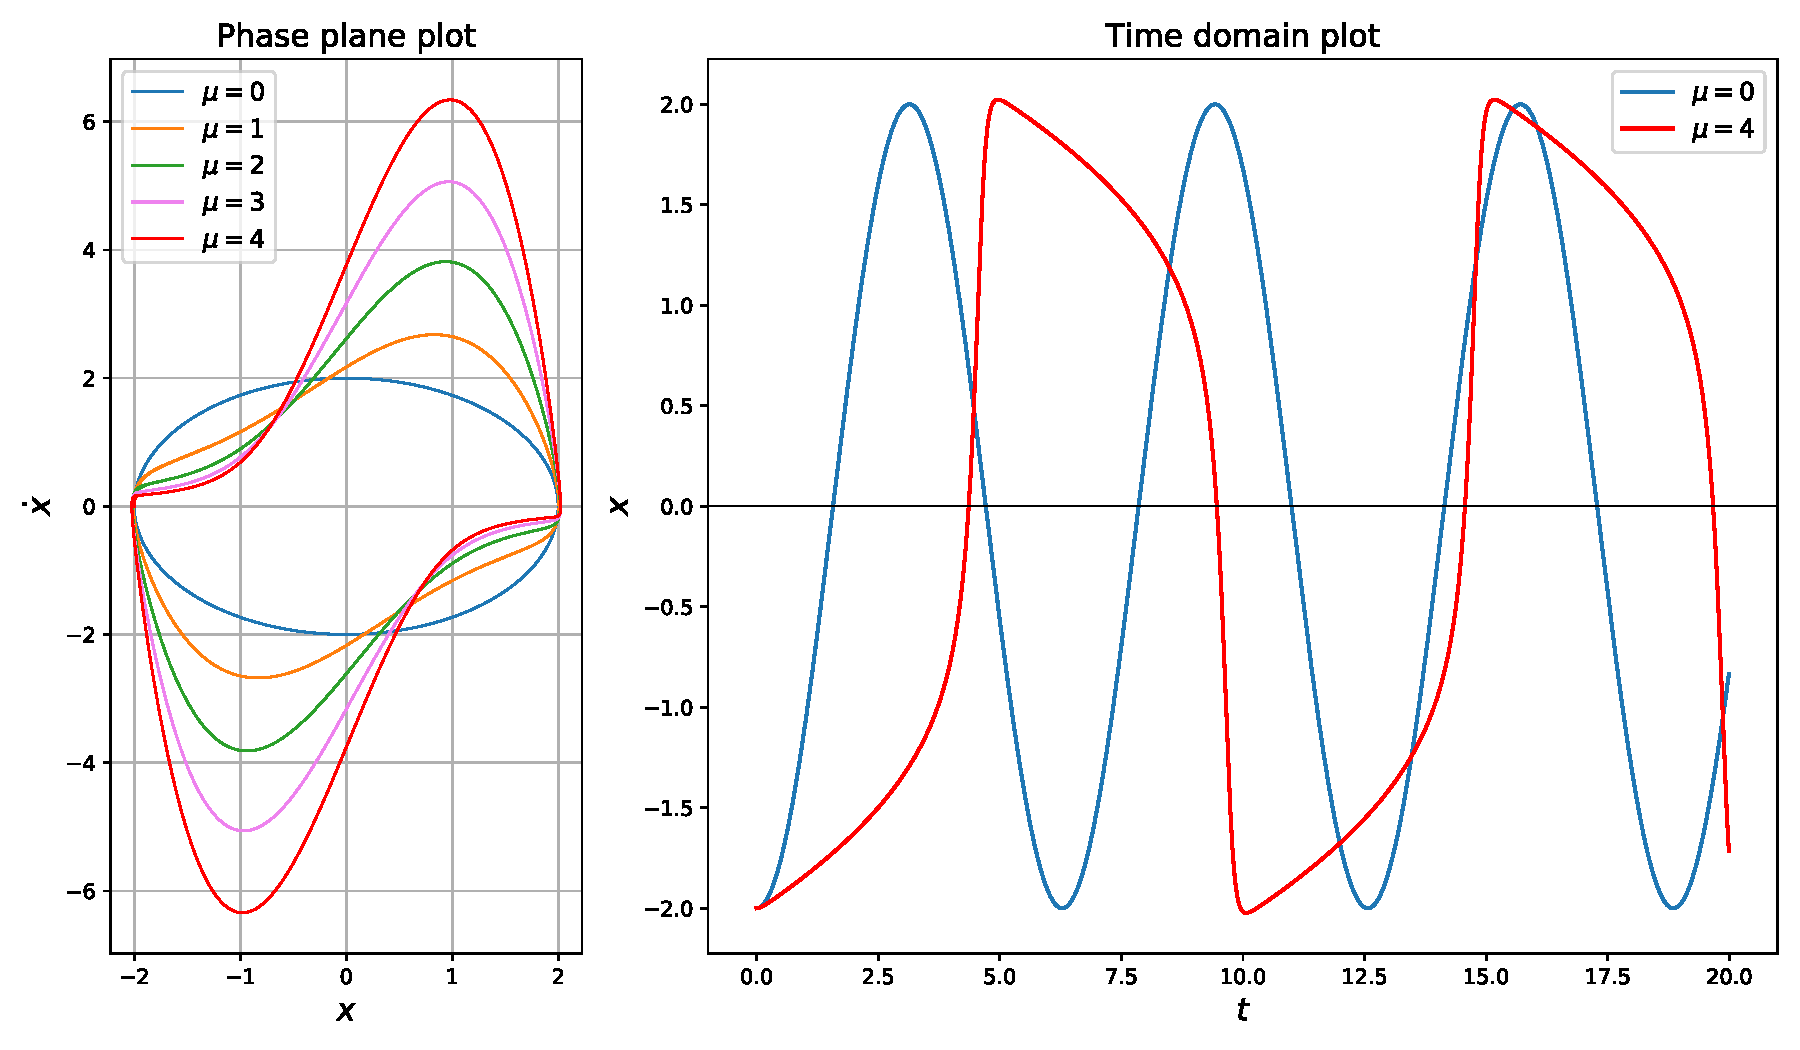
\includegraphics[width=\textwidth]{papers/vanderpol/figures/homogene_plot.pdf}
	\caption{Phase und Zeit-Raum-Diagramm mit verschiedenen $\mu$\label{vanderpol:figures:homogene}}
\end{figure}
Die homogene Van-der-Pol-Gleichung ist stabil und zeigt {\em kein} chaotisches Verhalten.
\subsection{Inhomogene Gleichung}
\label{vanderpol:subsection:inhomogene}
Um einen chaotischen Verlauf zu beobachten, ist es daher notwendig, die inhomogene Gleichung zu untersuchen:
\begin{equation*}
	\ddot{x}-\mu\left(1-x^{2}\right) \dot{x}+x = f(x)
\label{vanderpol:equations:inhomogene_gen}
\end{equation*}
Durch die Einstellung $f(x) = A \sin(\omega t)$ wird die Gleichung zur sogenannten {\em angeregte Van der Pol Gleichung}:
\begin{equation}
	\ddot{x}-\mu\left(1-x^{2}\right) \dot{x}+x = A \cdot \sin(\omega t)
\label{vanderpol:equations:inhomogene_sin}
\end{equation}
In der praktischen Anwendung ist es so, wie wenn man einen Wechselstromgenerator an den Oszillator anschliesst. Wie vorher geschehen (Gl. \ref{vanderpol:equations:homogene_1}), wird die Differentialgleichung auf die erste Ordnung reduziert:
\begin{align}
\frac{d}{dt}\begin{pmatrix}x \\ y\end{pmatrix} = \begin{pmatrix}y \\ \mu \left(1-x^{2}\right)\dot{x}-x+A \cdot \sin(\omega t)\end{pmatrix}
\label{vanderpol:equations:inhomogene_2}
\end{align}
Die Änderung der Amplitude $A$ verändert das Systemverhalten. Bei der Beobachtung der Frequenz des Oszillators wurden drei verschiedene Fälle erkannt. Wie in der Abb. \ref{vanderpol:figures:fft} gezeigt, ist die Frequenz des Van-der-Pol-Oszillators dominant, wenn der Wert $A$ kleiner als der kritische Wert ist. Wenn der Wert höher ist, dominiert die Frequenz $\omega$. Beim kritischen Punkt gibt es eine Summe von Frequenzen im System. Durch Setzen der Werte $\mu=0.2$ und $\omega=1.15$ beträgt der kritische Wert von $A$ in diesem Fall $0.32$. Wie in der folgenden Gleichung beschrieben:
\begin{equation}
	\ddot{x}-0.2\left(1-x^{2}\right) \dot{x}+x = A \cdot \sin(1.15 t)
	\label{vanderpol:equations:inhomogene_3}
\end{equation}


\begin{figure}
	\centering
	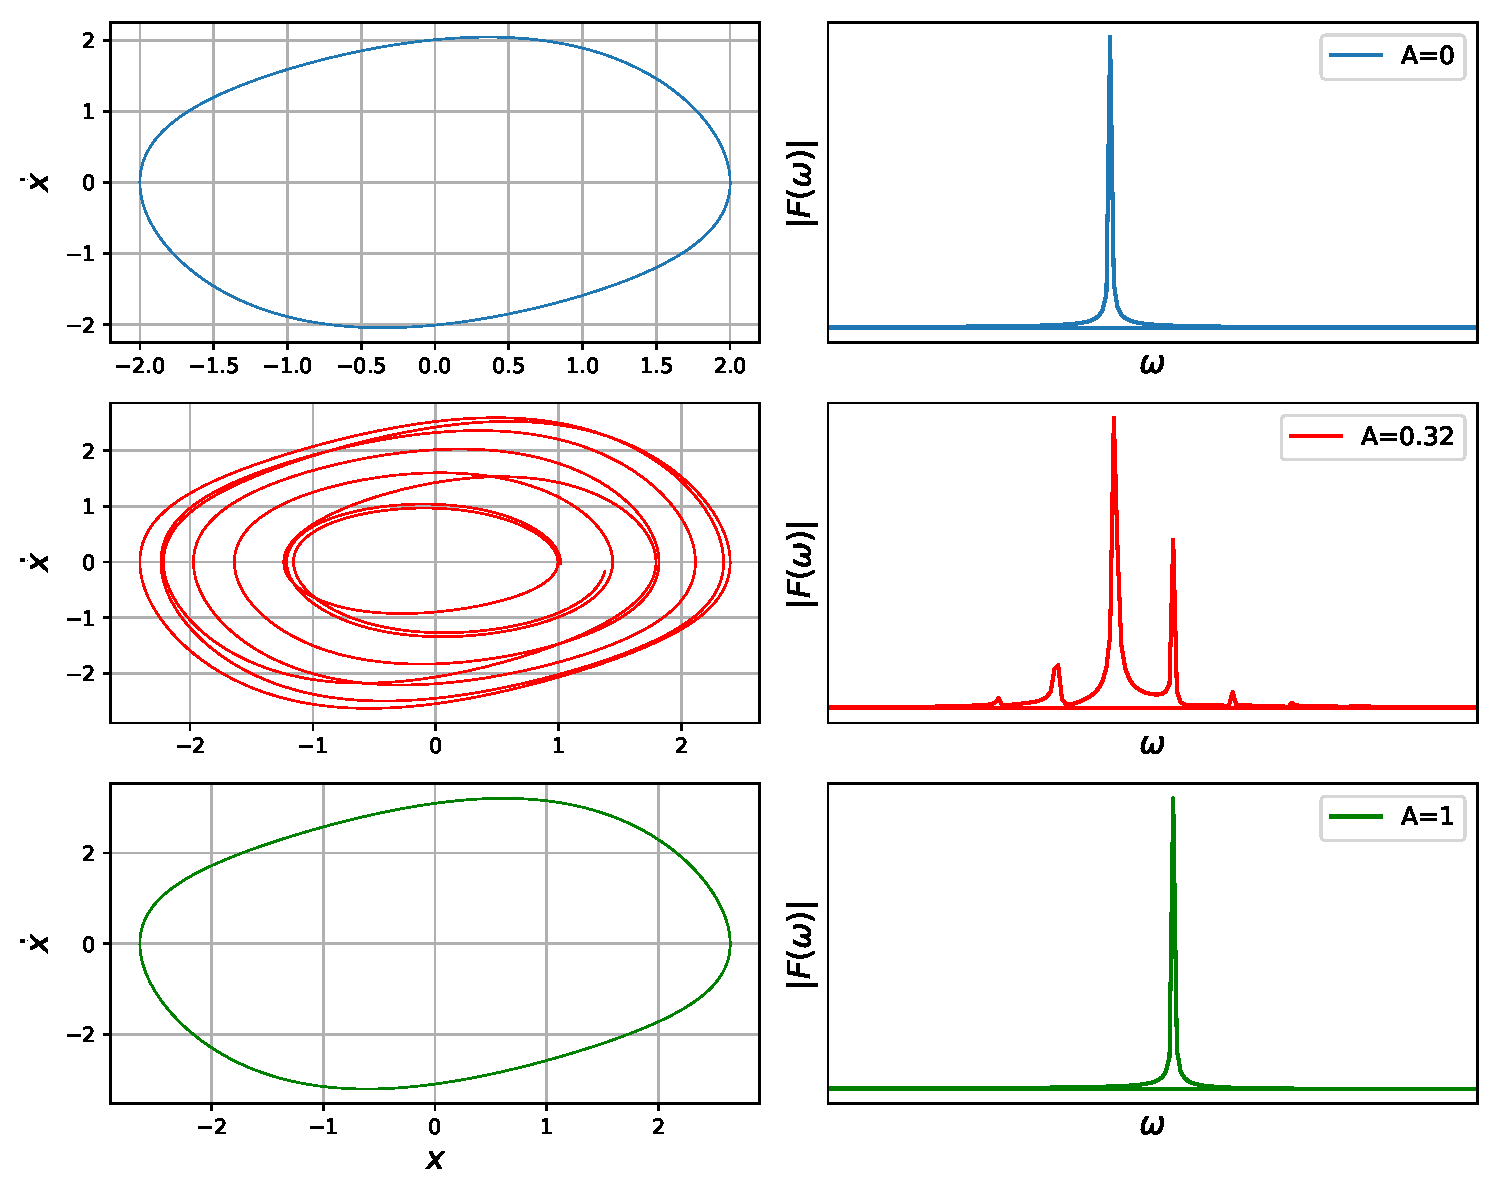
\includegraphics[width=0.9\textwidth]{papers/vanderpol/figures/fft_plot2.pdf}
	\caption{Phaseraum Diagramm und Frequenzspektrum der Gleichung \ref{vanderpol:equations:inhomogene_3} mit verschiedenen Werten von $A$.\label{vanderpol:figures:fft}}
\end{figure}

\subsection{Chaos}
\label{vanderpol:subsection:chaos}

\begin{cquote}[30pt]{Edward Lorenz}
``Chaos: When the present determines the future, but the approximate present does not approximately determine the future.''
\end{cquote}

\subsubsection{Anfangsbedingung}
\label{vanderpol:subsubsection:anfangsbedingung}
Das angeführte Zitat ist genau die Definition, die das in diesem Kapitel untersuchte Problem erklärt, nämlich die Instabilität der numerischen Methoden. Letztere führen zu einem Rundungsfehler, der sich während der verschiedenen Iterationen ansammelt. Diese hängt von der für den Integrationsschritt gewählten Länge ab. Mehrere Längen entsprechen daher unterschiedlichen Werten des Fehlers. Per Definition ist ein chaotisches System sehr empfindlich gegenüber Veränderungen, auch wenn diese minimal sind. Zwei Fehler aufgrund von zwei unterschiedlichen Integrationsschritten können somit zu zwei völlig unterschiedlichen Lösungen führen. In der Regel tritt die Divergenz zwischen den beiden Lösungen nach einer bestimmten Zeitspanne auf. Etwas Ähnliches geschieht, wenn, immer in einem chaotischen System, eine kleine Variation der Anfangsbedingungen eingeführt wird. Dieser kleine Unterschied kann, analog zu dem durch Fehler verursachten, das Langzeitverhalten des Systems stark beeinflussen. Diese Empfindlichkeit gegenüber Veränderungen im Ausgangszustand ist auch bekannt als {\em Butterfly Effect}. Zur Erklärung dieses Phänomens verwendete Edward Lorentz in 1972 auf einer Konferenz diesen Satz:\\``Ein Schmetterling schlägt in Peking mit den Flügeln, und in New York kommt Regen statt Sonne''.

\begin{wrapfigure}[14]{l}{0.4\textwidth}
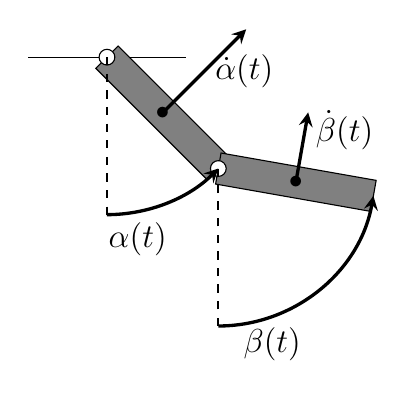
\begin{tikzpicture}[scale=1]

\draw (-1,0) -- (1,0);

\begin{scope}[rotate=45]

\draw[fill=gray]  (-0.2, 0) rectangle (0.2,-2.0) node[midway](a){$\bullet$};
%alpha'(t)
\draw[->, very thick, -stealth](0.0,-1.0) -- (1.5, -1.0) node[midway, right]{\large $\dot{\alpha}(t)$};

\draw[fill=gray, rotate around={35:(0, -2.0)}] (-0.2,-2.0) rectangle (0.2,-4.0)node[midway](a){$\bullet$};
%beta'(t)
\draw[->,very thick, -stealth, rotate around={35:(0, -2.0)}](0,-3.0) -- (0.9, -3.0) node[near end, above, right]{\large $\dot{\beta}(t)$};

\draw[fill=white] (0,-2.0) circle(0.1);
\draw[fill=white] (0,0) circle(0.1);

\end{scope}

\draw[very thick, ->, -stealth](0,-2.0) arc (-90:-45:2) node[near start, below]{\large $\alpha(t)$};
\draw[thick,dash pattern=on 3 off 3] (0,0) -- (0,-2.0);

\draw[very thick, ->, -stealth](1.414,-3.414) arc (-90:-10:2) node[near start, below]{\large $\beta(t)$};
\draw[thick,dash pattern=on 3 off 3] (1.414,-3.414)--(1.414,-1.414);

\end{tikzpicture}
\caption{Doppelpendel\label{vanderpol:figures:doublependulum}}
\end{wrapfigure}
\noindent Kann also eine solch minimale Veränderung der Anfangsbedingungen das Endergebnis vollständig verändern? Die Antwort ist offensichtlich ja, was auch durch die Grafiken auf den folgenden Seiten bewiesen wird.
Im Falle des Bildes Abb. \ref{vanderpol:figures:init_cond_dbl_pend} wurde die Lösung des hier links dargestellten Systems, ein Doppelpendel, berichtet. Es wird natürlich nicht im Detail behandelt, da dies nicht die Aufgabe dieses Kapitels ist. Es handelt sich jedoch um ein praktisches Beispiel, das genau zeigt, was im Anfangszitat zusammengefasst ist. Die beiden gezeigten Funktionen stellen den $\alpha$ Winkel zweier Doppelpendel mit Anfangsbedingungen dar, die eine geringe Abweichung aufweisen. Die Ausgangssituation wird also durch die folgenden Werte beschrieben:
\begin{itemize}
\item
$\alpha_1(0) = \frac{\pi}{2}$
\item
$\alpha_2(0) = \alpha_1(0) + \delta, \quad \delta = 10^{-3}$ 
\item
$\dot{\alpha_1}(0) = \dot{\alpha_2}(0)= 1 \frac{m}{s}, \quad \dot{\beta_1}(0) = \dot{\beta_2}(0)= 1 \frac{m}{s}, \quad \beta_1(0)=\beta_2(0)=\frac{\pi}{2}$
\end{itemize}

\begin{figure}
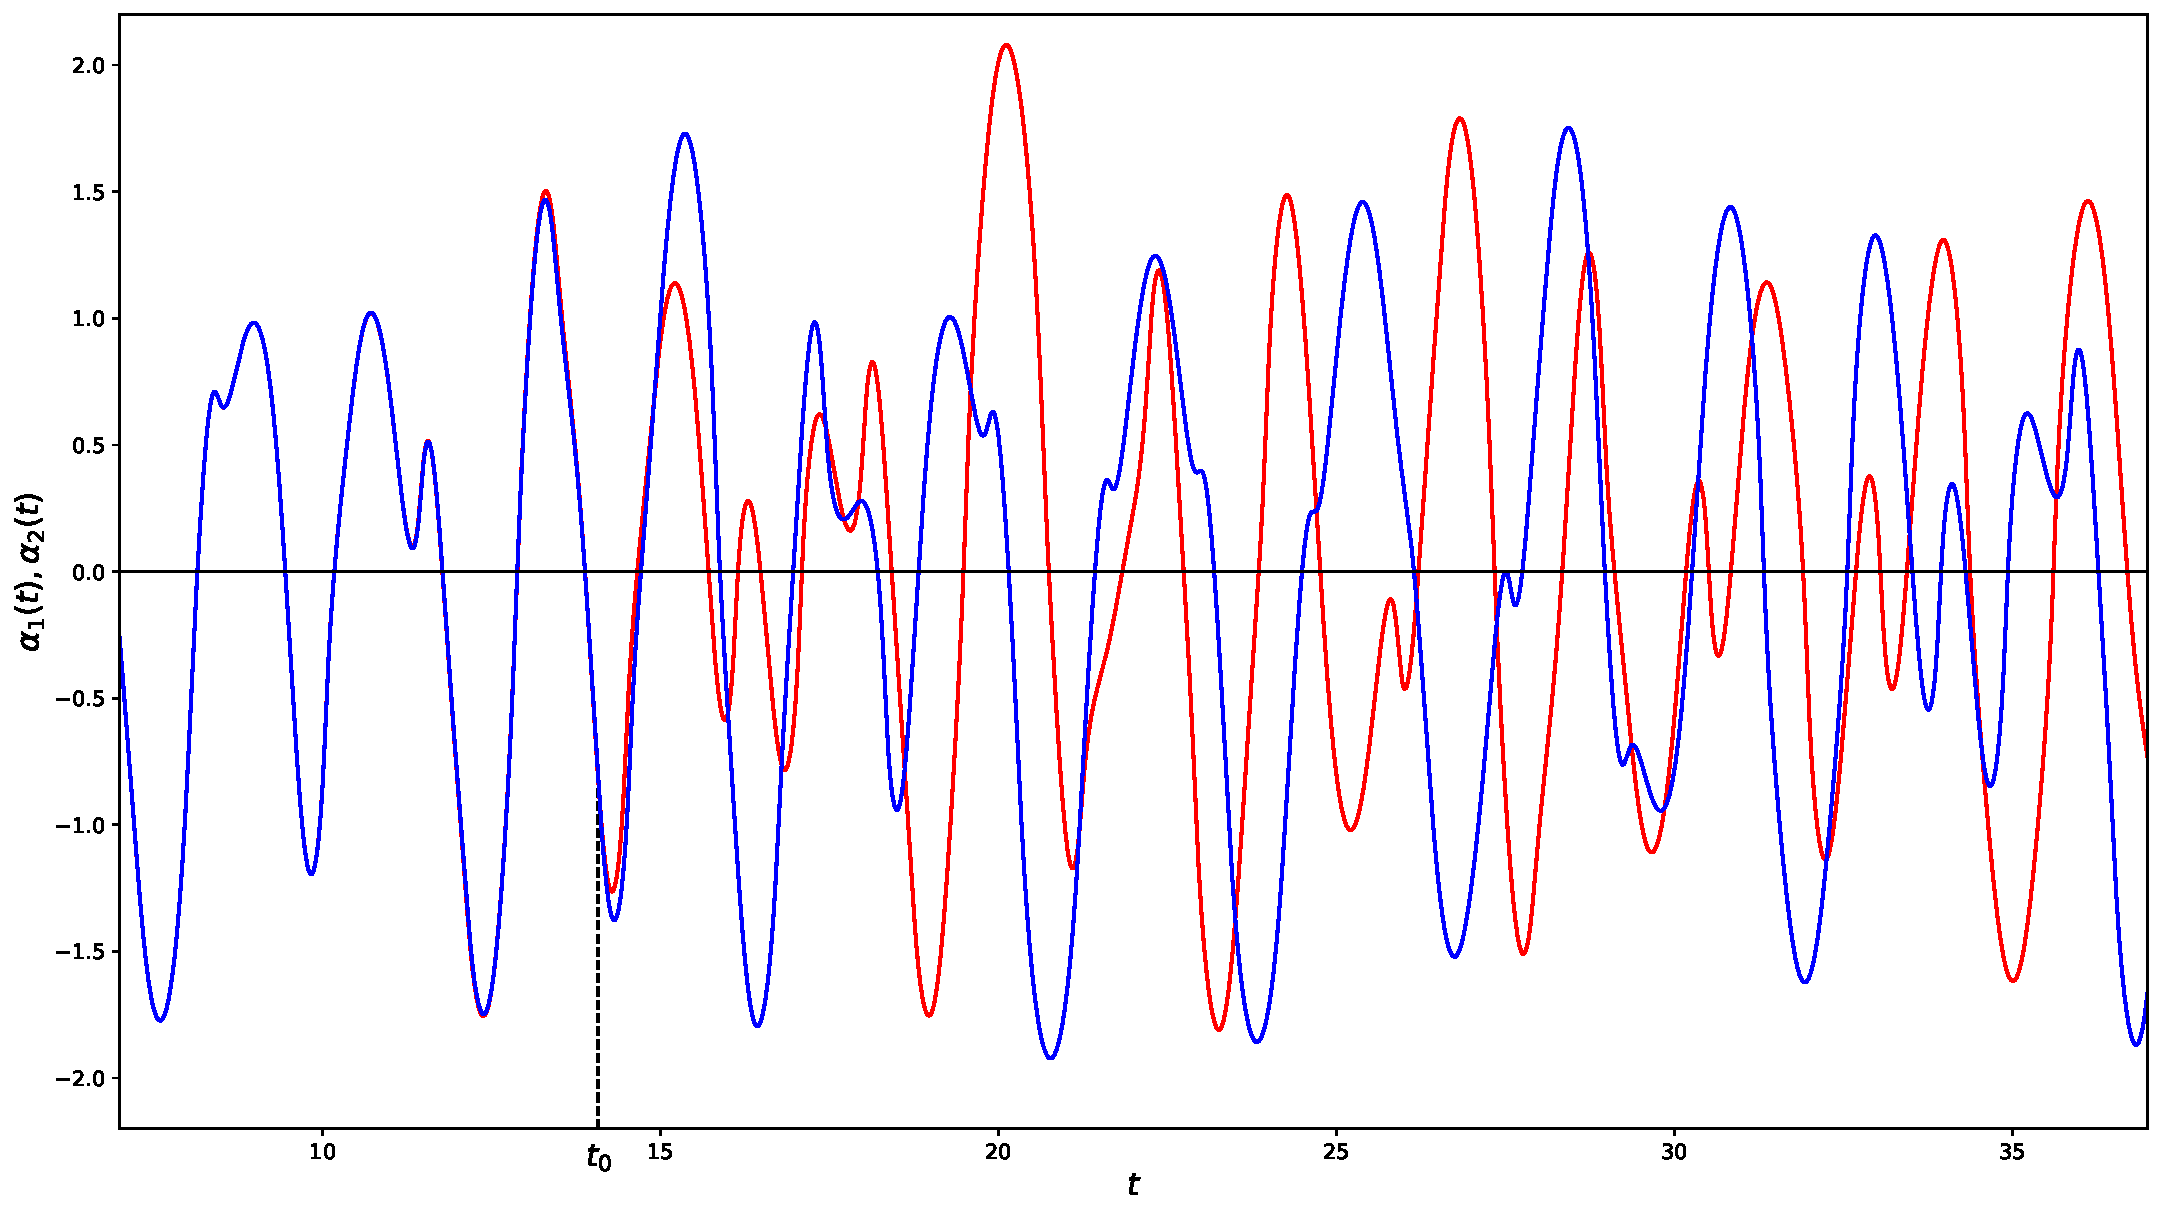
\includegraphics[width=\textwidth]{papers/vanderpol/figures/initial_cond_DBLPEND.pdf}
\caption{Winkelsverlauf $\alpha_1(t)$, $\alpha_2(t)$ und Angabe des Divergenzpunktes $t_0$ \label{vanderpol:figures:init_cond_dbl_pend}}
\end{figure}
\noindent Wie in Abb. \ref{vanderpol:figures:init_cond_dbl_pend} zu sehen ist, überlagern sich die beiden Lösungen im Anfangsmoment und sind nicht zu unterscheiden. Ab dem Punkt $t_0$ merkt man, dass sie plötzlich ganz andere Bahnen verfolgen. Die geringe anfängliche Varianz von $\delta$ hat daher die Endergebnisse in nicht gleichgültiger Weise beeinflusst. Dasselbe geschieht auch im Fall der Van der Pol-Gleichung. Im  Abb. \ref{vanderpol:figures:init_cond_VDP} sind zwei Darstellungen des Verlaufs der beiden mit dem gleichen Integrationsschritt erhaltenen numerischen Lösungen der Gl. \ref{vanderpol:equations:inhomogene_2} im Zeitbereich gezeigt. Die Anfangsbedingung sind in diesem Fall wie folgt gewählt worden:

\begin{figure}
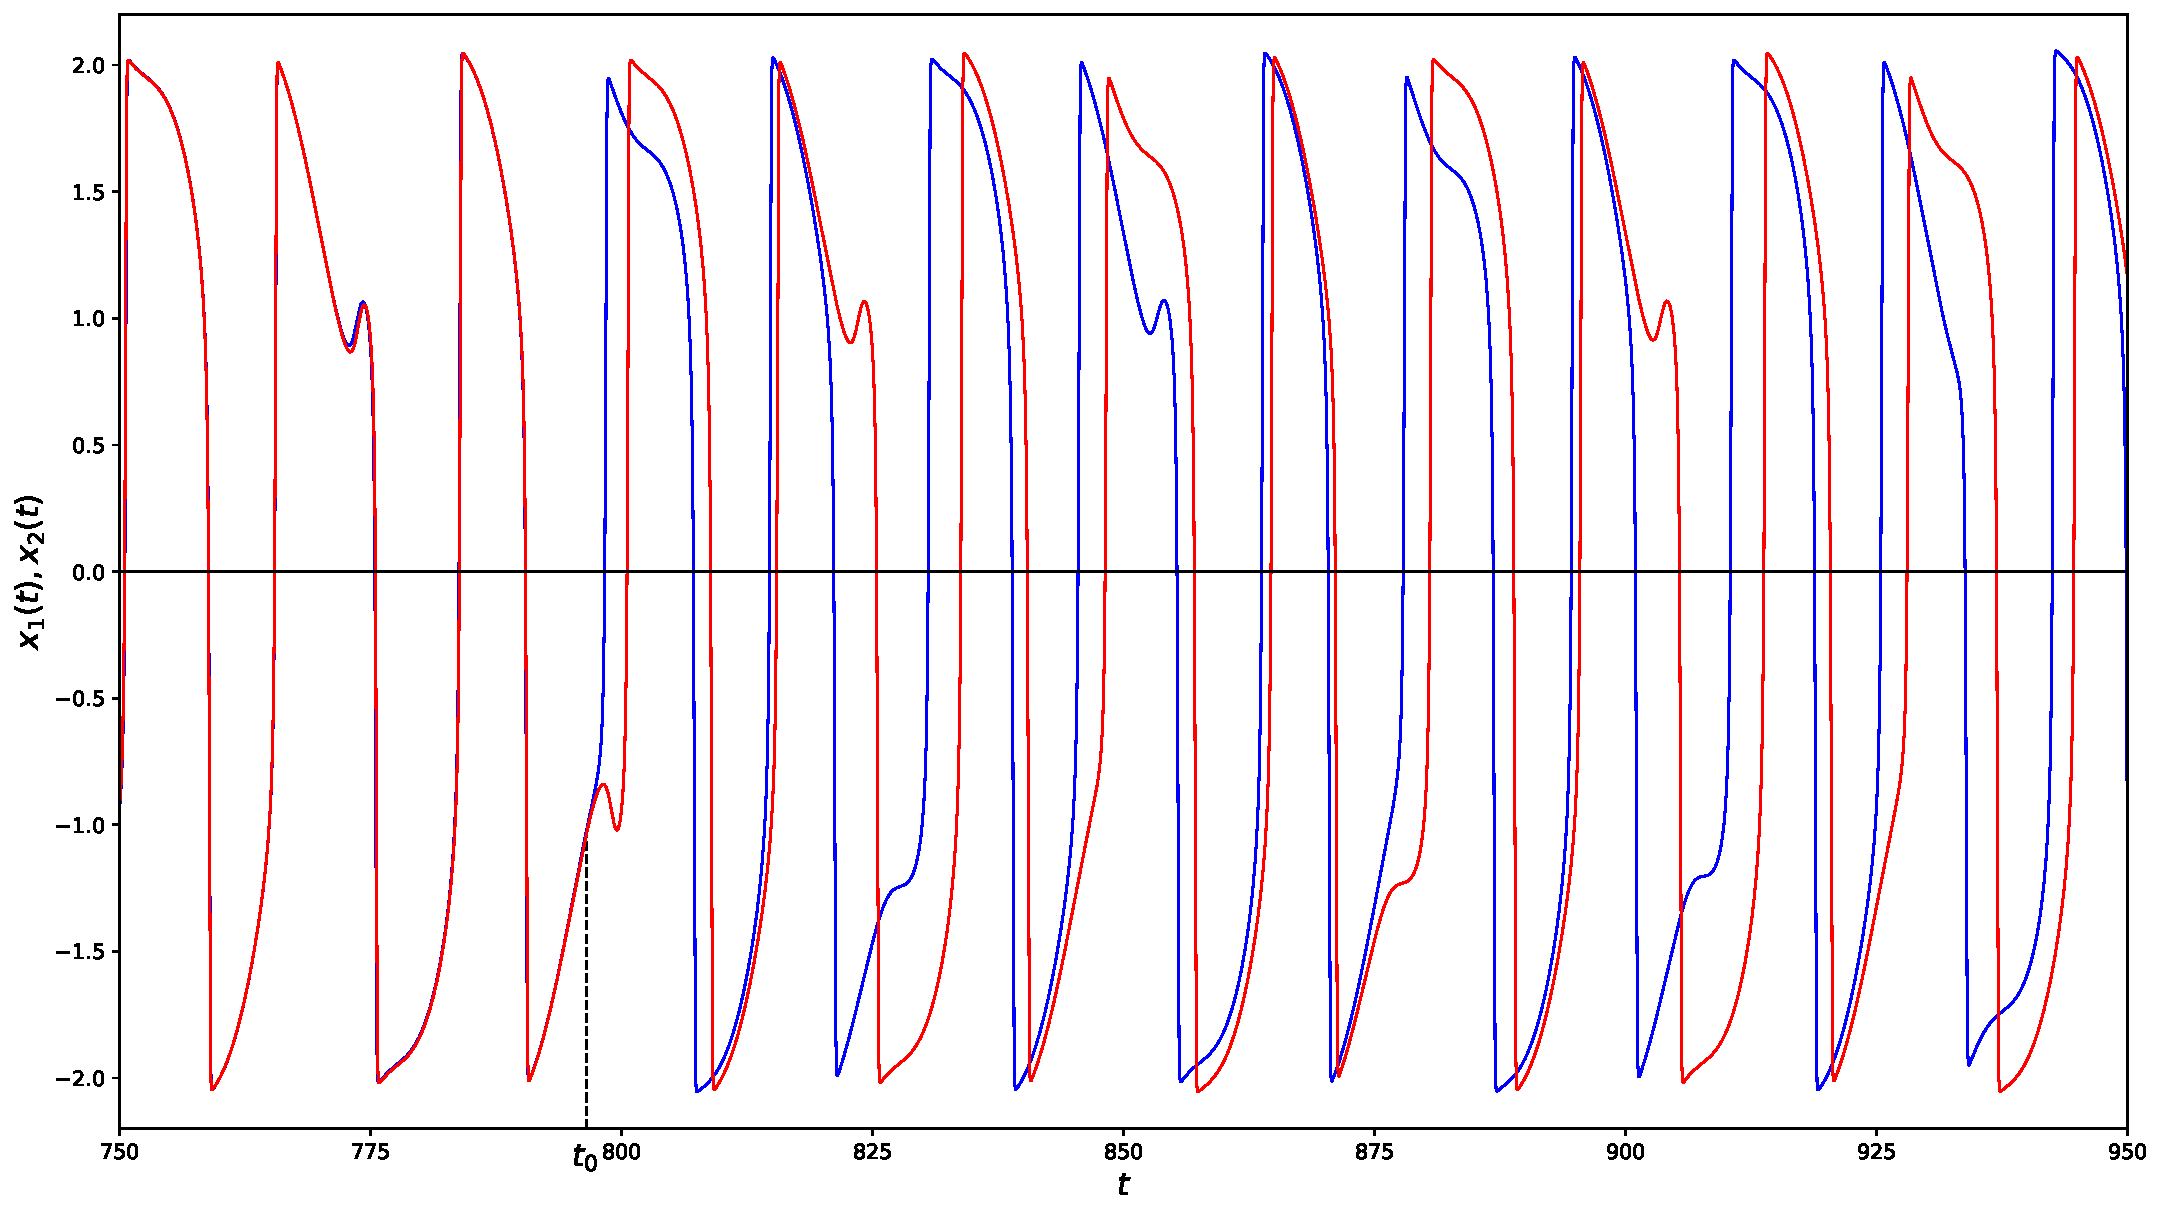
\includegraphics[width=\textwidth]{papers/vanderpol/figures/initial_cond_VDP.pdf}
\caption{Lösungsverlauf $x_1(t)$, $x_2(t)$ und Angabe des Divergenzpunktes $t_0$ \label{vanderpol:figures:init_cond_VDP}}
\end{figure}

\begin{itemize}
\item
$\dot{x_1}(0) = 5$
\item
$\dot{x_1}(0) = \dot{x_1}(0) + \delta, \quad \delta = 10^{-3}$ 
\item
$x_1(0) = x_2(0) = 0$
\end{itemize}
Daraus lässt sich natürlich schliessen, dass beide Systeme aufgrund ihrer chaotischen Natur sehr empfindlich auf die Anfangsbedingungen reagieren. Dies lässt sich auf den Ausgangskurs zurückführen, denn im Falle einer numerischen, nämlich eine approximativen Lösung $\hat{y}$, gilt dass:

\begin{equation} 
\mid \hat{y}(x_n) - y(x_n) \mid = \epsilon
\end{equation}
Obwohl $\epsilon$ ein sehr kleiner Wert sein kann, kann er unter bestimmten Umständen die gleiche Wirkung haben wie eine Änderung der Anfangsbedingungen. Dank der beiden Diagramme Abb.   \ref{vanderpol:figures:init_cond_VDP} und Abb. \ref{vanderpol:figures:init_cond_dbl_pend} konnte man feststellen, dass der Unterschied zwar in der Grössenordnung von $10^{-3}$ lag, aber nach einiger Zeit zu einer völlig anderen Topologie führte. Wie im nächsten Kapitel erläutert, gilt dies auch für die Änderung des Integrationsschrittes.